\documentclass{extbook}[14pt]
\usepackage{multicol, enumerate, enumitem, hyperref, color, soul, setspace, parskip, fancyhdr, amssymb, amsthm, amsmath, latexsym, units, mathtools}
\everymath{\displaystyle}
\usepackage[headsep=0.5cm,headheight=0cm, left=1 in,right= 1 in,top= 1 in,bottom= 1 in]{geometry}
\usepackage{dashrule}  % Package to use the command below to create lines between items
\newcommand{\litem}[1]{\item #1

\rule{\textwidth}{0.4pt}}
\pagestyle{fancy}
\lhead{}
\chead{Answer Key for Progress Quiz 6 Version A}
\rhead{}
\lfoot{4563-7456}
\cfoot{}
\rfoot{Summer C 2021}
\begin{document}
\textbf{This key should allow you to understand why you choose the option you did (beyond just getting a question right or wrong). \href{https://xronos.clas.ufl.edu/mac1105spring2020/courseDescriptionAndMisc/Exams/LearningFromResults}{More instructions on how to use this key can be found here}.}

\textbf{If you have a suggestion to make the keys better, \href{https://forms.gle/CZkbZmPbC9XALEE88}{please fill out the short survey here}.}

\textit{Note: This key is auto-generated and may contain issues and/or errors. The keys are reviewed after each exam to ensure grading is done accurately. If there are issues (like duplicate options), they are noted in the offline gradebook. The keys are a work-in-progress to give students as many resources to improve as possible.}

\rule{\textwidth}{0.4pt}

\begin{enumerate}\litem{
Construct the lowest-degree polynomial given the zeros below. Then, choose the intervals that contain the coefficients of the polynomial in the form $x^3+bx^2+cx+d$.
\[ -3 - 2 i \text{ and } -3 \]The solution is \( x^{3} +9 x^{2} +31 x + 39 \), which is option C.\begin{enumerate}[label=\Alph*.]
\item \( b \in [-5, 3], c \in [5.4, 6.45], \text{ and } d \in [7.9, 9.4] \)

$x^{3} + x^{2} +6 x + 9$, which corresponds to multiplying out $(x + 3)(x + 3)$.
\item \( b \in [-5, 3], c \in [4.58, 5.53], \text{ and } d \in [1.9, 7.1] \)

$x^{3} + x^{2} +5 x + 6$, which corresponds to multiplying out $(x + 2)(x + 3)$.
\item \( b \in [2, 13], c \in [30.15, 31.6], \text{ and } d \in [38.1, 39.8] \)

* $x^{3} +9 x^{2} +31 x + 39$, which is the correct option.
\item \( b \in [-17, -6], c \in [30.15, 31.6], \text{ and } d \in [-42, -38.7] \)

$x^{3} -9 x^{2} +31 x -39$, which corresponds to multiplying out $(x-(-3 - 2 i))(x-(-3 + 2 i))(x -3)$.
\item \( \text{None of the above.} \)

This corresponds to making an unanticipated error or not understanding how to use nonreal complex numbers to create the lowest-degree polynomial. If you chose this and are not sure what you did wrong, please contact the coordinator for help.
\end{enumerate}

\textbf{General Comment:} Remember that the conjugate of $a+bi$ is $a-bi$. Since these zeros always come in pairs, we need to multiply out $(x-(-3 - 2 i))(x-(-3 + 2 i))(x-(-3))$.
}
\litem{
Which of the following equations \textit{could} be of the graph presented below?

\begin{center}
    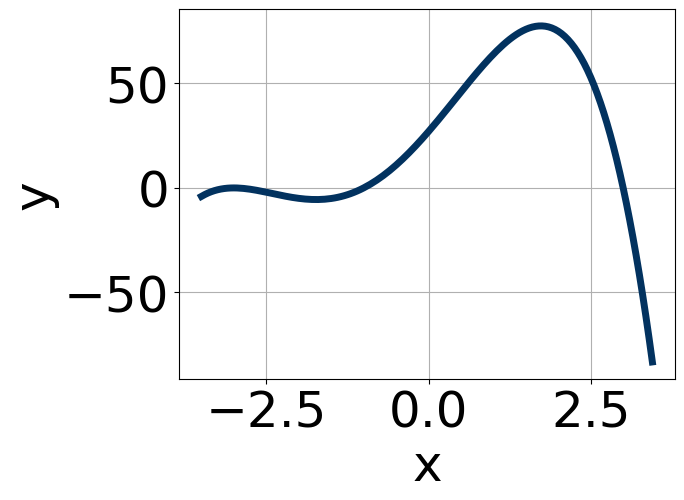
\includegraphics[width=0.5\textwidth]{../Figures/polyGraphToFunctionA.png}
\end{center}


The solution is \( -15(x + 3)^{10} (x - 3)^{7} (x + 1)^{11} \), which is option A.\begin{enumerate}[label=\Alph*.]
\item \( -15(x + 3)^{10} (x - 3)^{7} (x + 1)^{11} \)

* This is the correct option.
\item \( -9(x + 3)^{11} (x - 3)^{8} (x + 1)^{9} \)

The factor $-3$ should have an even power and the factor $3$ should have an odd power.
\item \( -7(x + 3)^{10} (x - 3)^{6} (x + 1)^{7} \)

The factor $(x - 3)$ should have an odd power.
\item \( 5(x + 3)^{10} (x - 3)^{5} (x + 1)^{4} \)

The factor $(x + 1)$ should have an odd power and the leading coefficient should be the opposite sign.
\item \( 7(x + 3)^{6} (x - 3)^{5} (x + 1)^{5} \)

This corresponds to the leading coefficient being the opposite value than it should be.
\end{enumerate}

\textbf{General Comment:} General Comments: Draw the x-axis to determine which zeros are touching (and so have even multiplicity) or cross (and have odd multiplicity).
}
\litem{
Which of the following equations \textit{could} be of the graph presented below?

\begin{center}
    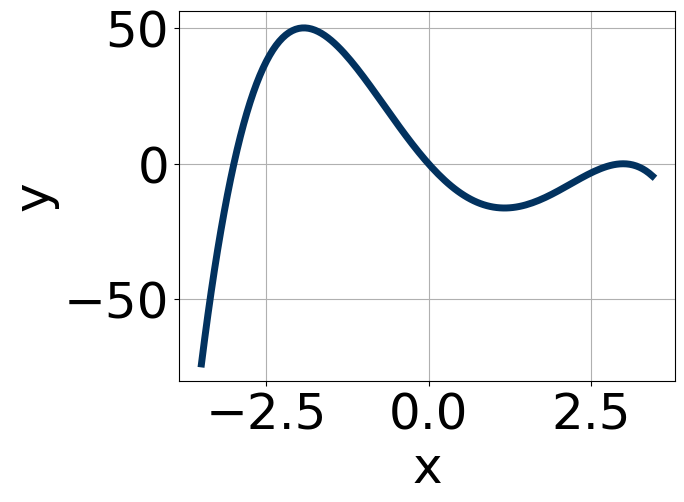
\includegraphics[width=0.5\textwidth]{../Figures/polyGraphToFunctionCopyA.png}
\end{center}


The solution is \( -7x^{7} (x - 3)^{8} (x + 3)^{5} \), which is option D.\begin{enumerate}[label=\Alph*.]
\item \( 10x^{7} (x - 3)^{4} (x + 3)^{10} \)

The factor $(x + 3)$ should have an odd power and the leading coefficient should be the opposite sign.
\item \( 15x^{11} (x - 3)^{6} (x + 3)^{5} \)

This corresponds to the leading coefficient being the opposite value than it should be.
\item \( -20x^{6} (x - 3)^{9} (x + 3)^{7} \)

The factor $3$ should have an even power and the factor $0$ should have an odd power.
\item \( -7x^{7} (x - 3)^{8} (x + 3)^{5} \)

* This is the correct option.
\item \( -18x^{4} (x - 3)^{4} (x + 3)^{5} \)

The factor $x$ should have an odd power.
\end{enumerate}

\textbf{General Comment:} General Comments: Draw the x-axis to determine which zeros are touching (and so have even multiplicity) or cross (and have odd multiplicity).
}
\litem{
Describe the zero behavior of the zero $x = 4$ of the polynomial below.
\[ f(x) = 2(x + 6)^{8}(x - 6)^{4}(x - 4)^{10}(x + 4)^{7} \]The solution is the graph below, which is option C.
    \begin{center}
        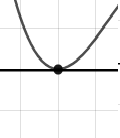
\includegraphics[width=0.3\textwidth]{../Figures/polyZeroBehaviorCopyCA.png}
    \end{center}\begin{enumerate}[label=\Alph*.]
\begin{multicols}{2}
\item 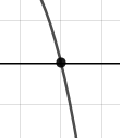
\includegraphics[width = 0.3\textwidth]{../Figures/polyZeroBehaviorCopyAA.png}
\item 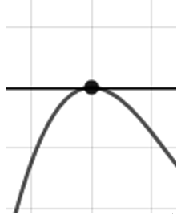
\includegraphics[width = 0.3\textwidth]{../Figures/polyZeroBehaviorCopyBA.png}
\item 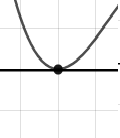
\includegraphics[width = 0.3\textwidth]{../Figures/polyZeroBehaviorCopyCA.png}
\item 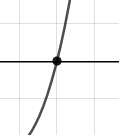
\includegraphics[width = 0.3\textwidth]{../Figures/polyZeroBehaviorCopyDA.png}
\end{multicols}\item None of the above.\end{enumerate}
\textbf{General Comment:} You will need to sketch the entire graph, then zoom in on the zero the question asks about.
}
\litem{
Construct the lowest-degree polynomial given the zeros below. Then, choose the intervals that contain the coefficients of the polynomial in the form $x^3+bx^2+cx+d$.
\[ 2 + 3 i \text{ and } 3 \]The solution is \( x^{3} -7 x^{2} +25 x -39 \), which is option D.\begin{enumerate}[label=\Alph*.]
\item \( b \in [4, 11], c \in [21.54, 25.63], \text{ and } d \in [33, 43] \)

$x^{3} +7 x^{2} +25 x + 39$, which corresponds to multiplying out $(x-(2 + 3 i))(x-(2 - 3 i))(x + 3)$.
\item \( b \in [-3, 5], c \in [-5.17, -2.87], \text{ and } d \in [0, 7] \)

$x^{3} + x^{2} -5 x + 6$, which corresponds to multiplying out $(x -2)(x -3)$.
\item \( b \in [-3, 5], c \in [-6.83, -5.89], \text{ and } d \in [9, 10] \)

$x^{3} + x^{2} -6 x + 9$, which corresponds to multiplying out $(x -3)(x -3)$.
\item \( b \in [-9, -4], c \in [21.54, 25.63], \text{ and } d \in [-46, -38] \)

* $x^{3} -7 x^{2} +25 x -39$, which is the correct option.
\item \( \text{None of the above.} \)

This corresponds to making an unanticipated error or not understanding how to use nonreal complex numbers to create the lowest-degree polynomial. If you chose this and are not sure what you did wrong, please contact the coordinator for help.
\end{enumerate}

\textbf{General Comment:} Remember that the conjugate of $a+bi$ is $a-bi$. Since these zeros always come in pairs, we need to multiply out $(x-(2 + 3 i))(x-(2 - 3 i))(x-(3))$.
}
\litem{
Construct the lowest-degree polynomial given the zeros below. Then, choose the intervals that contain the coefficients of the polynomial in the form $ax^3+bx^2+cx+d$.
\[ \frac{3}{5}, \frac{-1}{3}, \text{ and } \frac{-1}{2} \]The solution is \( 30x^{3} +7 x^{2} -10 x -3 \), which is option E.\begin{enumerate}[label=\Alph*.]
\item \( a \in [30, 39], b \in [-13, -1], c \in [-13, -6], \text{ and } d \in [-1, 7] \)

$30x^{3} -7 x^{2} -10 x + 3$, which corresponds to multiplying out $(5x + 3)(3x -1)(2x -1)$.
\item \( a \in [30, 39], b \in [40, 44], c \in [18, 24], \text{ and } d \in [-1, 7] \)

$30x^{3} +43 x^{2} +20 x + 3$, which corresponds to multiplying out $(5x + 3)(3x + 1)(2x + 1)$.
\item \( a \in [30, 39], b \in [22, 27], c \in [-2, 0], \text{ and } d \in [-3, -2] \)

$30x^{3} +23 x^{2} -2 x -3$, which corresponds to multiplying out $(5x + 3)(3x -1)(2x + 1)$.
\item \( a \in [30, 39], b \in [7, 13], c \in [-13, -6], \text{ and } d \in [-1, 7] \)

$30x^{3} +7 x^{2} -10 x + 3$, which corresponds to multiplying everything correctly except the constant term.
\item \( a \in [30, 39], b \in [7, 13], c \in [-13, -6], \text{ and } d \in [-3, -2] \)

* $30x^{3} +7 x^{2} -10 x -3$, which is the correct option.
\end{enumerate}

\textbf{General Comment:} To construct the lowest-degree polynomial, you want to multiply out $(5x -3)(3x + 1)(2x + 1)$
}
\litem{
Describe the end behavior of the polynomial below.
\[ f(x) = -7(x - 9)^{5}(x + 9)^{8}(x + 4)^{5}(x - 4)^{7} \]The solution is the graph below, which is option A.
    \begin{center}
        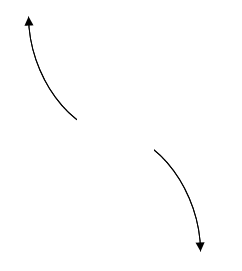
\includegraphics[width=0.3\textwidth]{../Figures/polyEndBehaviorAA.png}
    \end{center}\begin{enumerate}[label=\Alph*.]
\begin{multicols}{2}
\item 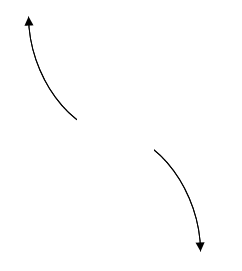
\includegraphics[width = 0.3\textwidth]{../Figures/polyEndBehaviorAA.png}
\item 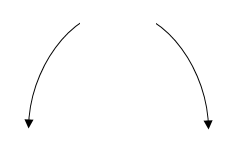
\includegraphics[width = 0.3\textwidth]{../Figures/polyEndBehaviorBA.png}
\item 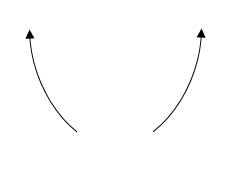
\includegraphics[width = 0.3\textwidth]{../Figures/polyEndBehaviorCA.png}
\item 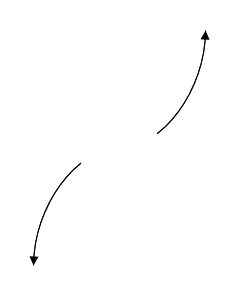
\includegraphics[width = 0.3\textwidth]{../Figures/polyEndBehaviorDA.png}
\end{multicols}\item None of the above.\end{enumerate}
\textbf{General Comment:} Remember that end behavior is determined by the leading coefficient AND whether the \textbf{sum} of the multiplicities is positive or negative.
}
\litem{
Construct the lowest-degree polynomial given the zeros below. Then, choose the intervals that contain the coefficients of the polynomial in the form $ax^3+bx^2+cx+d$.
\[ \frac{-6}{5}, \frac{3}{5}, \text{ and } \frac{7}{2} \]The solution is \( 50x^{3} -145 x^{2} -141 x + 126 \), which is option E.\begin{enumerate}[label=\Alph*.]
\item \( a \in [48, 54], b \in [-154, -139], c \in [-141, -135], \text{ and } d \in [-128, -118] \)

$50x^{3} -145 x^{2} -141 x -126$, which corresponds to multiplying everything correctly except the constant term.
\item \( a \in [48, 54], b \in [-206, -201], c \in [67, 73], \text{ and } d \in [125, 132] \)

$50x^{3} -205 x^{2} +69 x + 126$, which corresponds to multiplying out $(5x -6)(5x + 3)(2x -7)$.
\item \( a \in [48, 54], b \in [-267, -261], c \in [350, 357], \text{ and } d \in [-128, -118] \)

$50x^{3} -265 x^{2} +351 x -126$, which corresponds to multiplying out $(5x -6)(5x -3)(2x -7)$.
\item \( a \in [48, 54], b \in [142, 152], c \in [-141, -135], \text{ and } d \in [-128, -118] \)

$50x^{3} +145 x^{2} -141 x -126$, which corresponds to multiplying out $(5x -6)(5x + 3)(2x + 7)$.
\item \( a \in [48, 54], b \in [-154, -139], c \in [-141, -135], \text{ and } d \in [125, 132] \)

* $50x^{3} -145 x^{2} -141 x + 126$, which is the correct option.
\end{enumerate}

\textbf{General Comment:} To construct the lowest-degree polynomial, you want to multiply out $(5x + 6)(5x -3)(2x -7)$
}
\litem{
Describe the zero behavior of the zero $x = 5$ of the polynomial below.
\[ f(x) = -7(x - 3)^{6}(x + 3)^{3}(x - 5)^{10}(x + 5)^{7} \]The solution is the graph below, which is option B.
    \begin{center}
        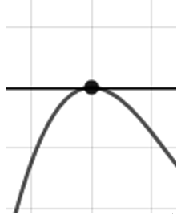
\includegraphics[width=0.3\textwidth]{../Figures/polyZeroBehaviorBA.png}
    \end{center}\begin{enumerate}[label=\Alph*.]
\begin{multicols}{2}
\item 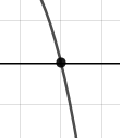
\includegraphics[width = 0.3\textwidth]{../Figures/polyZeroBehaviorAA.png}
\item 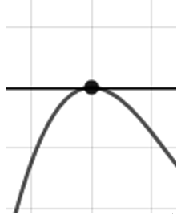
\includegraphics[width = 0.3\textwidth]{../Figures/polyZeroBehaviorBA.png}
\item 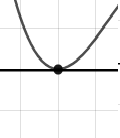
\includegraphics[width = 0.3\textwidth]{../Figures/polyZeroBehaviorCA.png}
\item 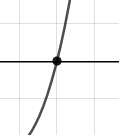
\includegraphics[width = 0.3\textwidth]{../Figures/polyZeroBehaviorDA.png}
\end{multicols}\item None of the above.\end{enumerate}
\textbf{General Comment:} You will need to sketch the entire graph, then zoom in on the zero the question asks about.
}
\litem{
Describe the end behavior of the polynomial below.
\[ f(x) = -8(x + 3)^{4}(x - 3)^{5}(x + 7)^{3}(x - 7)^{5} \]The solution is the graph below, which is option A.
    \begin{center}
        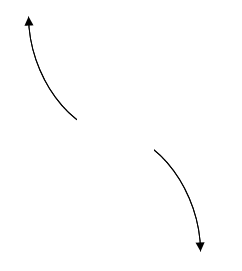
\includegraphics[width=0.3\textwidth]{../Figures/polyEndBehaviorCopyAA.png}
    \end{center}\begin{enumerate}[label=\Alph*.]
\begin{multicols}{2}
\item 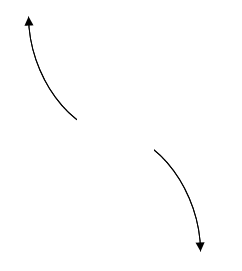
\includegraphics[width = 0.3\textwidth]{../Figures/polyEndBehaviorCopyAA.png}
\item 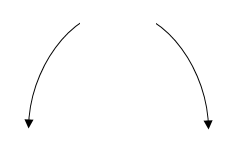
\includegraphics[width = 0.3\textwidth]{../Figures/polyEndBehaviorCopyBA.png}
\item 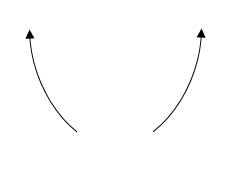
\includegraphics[width = 0.3\textwidth]{../Figures/polyEndBehaviorCopyCA.png}
\item 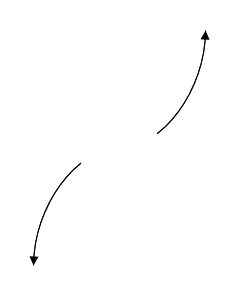
\includegraphics[width = 0.3\textwidth]{../Figures/polyEndBehaviorCopyDA.png}
\end{multicols}\item None of the above.\end{enumerate}
\textbf{General Comment:} Remember that end behavior is determined by the leading coefficient AND whether the \textbf{sum} of the multiplicities is positive or negative.
}
\end{enumerate}

\end{document}